\documentclass[11pt]{article}
\usepackage[T1]{fontenc}
\usepackage[utf8]{inputenc}
\usepackage{charter}
\usepackage[scaled=0.92]{helvet}
\renewcommand{\ttdefault}{lmtt}
\usepackage{amsmath}
\usepackage[margin=1in]{geometry}
\usepackage{booktabs}
\usepackage{graphicx}
\usepackage{microtype}
\usepackage{xcolor}
\usepackage[font=small,labelfont=bf,labelsep=period]{caption}
\usepackage{enumitem}
\usepackage[hidelinks]{hyperref}
\definecolor{link}{HTML}{1F3A7A}
\hypersetup{colorlinks=true,linkcolor=link,urlcolor=link,citecolor=link}
\setlist{nosep,leftmargin=1.4em}
\graphicspath{{../backtest/results/ml/}{../cpp/itch/results/}}
\newcommand{\dol}{\$}

\title{\textbf{Market Making on Apple's Order Book,\\ With and Without an Order-Flow Filter}}
\author{Adam Nguyen\\[2pt]
\small University of Washington, Mathematics and Informatics\\[1pt]
\small \href{https://orderbook-eosin.vercel.app/playground.html}{orderbook-eosin.vercel.app} \quad
\href{https://github.com/adamdn-code/orderbook}{github.com/adamdn-code/orderbook}}
\date{November 2026}

\begin{document}
\maketitle

\begin{abstract}
\noindent A market maker quotes Apple (AAPL) on a full day of real Nasdaq order flow, rebuilt message by message from the TotalView-ITCH feed by a C++ limit order book, with the queue position of every quote tracked exactly. A gradient-boosted model of the direction of the next mid-price move, trained on 19 causal order-flow features, reaches a test AUC of 0.652 on a held-out afternoon against 0.603 for book imbalance (gain $+0.048$, 95\% block-bootstrap interval $+0.041$ to $+0.054$). Used as a quote filter, with every threshold and activity rate chosen on a tuning hour before the test afternoon is run, it cuts the afternoon's loss from $-\dol1{,}147$ to $-\dol470$ at zero latency, and the ML filters lose less per share than imbalance in 126 of 132 settings at matched activity. With every model and setting frozen, a second day eleven months later gives AUC 0.648 against 0.605, and a fill-toxicity filter loses least at every latency. No configuration is profitable out of sample: the filters reduce adverse selection rather than create an edge.
\end{abstract}

\section{Introduction}
A passive market maker earns the spread on uninformed flow and loses to traders who know where the price is going. On a liquid stock with a one-cent spread the second effect dominates: the orders that fill a resting quote are disproportionately the ones about to move the price through it. The question here is narrow and testable: can a short-horizon model of the next price move, built only from the public order book, tell the market maker when to step out of the way, and does that survive honest out-of-sample evaluation, realistic latency, and a different day?

Three things make the answer credible rather than suggestive. The book is rebuilt from Nasdaq's own message log and checked against it (Section~\ref{sec:data}). Fills are simulated with exact queue position, not a probability model (Section~\ref{sec:mm}). And every choice that could be tuned, including the model's hyperparameters, the filter's threshold and how often it fires, is made on data before the test period, which is then run once.

\section{Data and the order book}\label{sec:data}
The data are Nasdaq's public TotalView-ITCH~5.0 sample files: every order added, executed, cancelled or replaced on Nasdaq for a full trading day. The primary day is 30~January~2019 (368 million messages, 8{,}695 stocks); the out-of-sample day is 30~December~2019.

\paragraph{The book.} A C++17 limit order book written for this project stores price levels in a flat array indexed by price, keeps a bitmap of non-empty levels so the next best price is found with one count-leading-zeros instruction, links orders into their levels' FIFO queues by index in a pooled vector, and maps order ids to slots with an open-addressing hash table. Nothing allocates once warm. On one thread it processes 6.1 million random orders per second with a 99th-percentile latency of 352~ns, against 2.9 million and 1{,}127~ns for a first version built on \texttt{std::map}; a randomized test requires the two to agree on every trade and every level after each of 300k operations. A multithreaded engine around it, with one matching thread per symbol and a lock-free single-producer, single-consumer ring per client per symbol, sustains 12.8 million orders per second from 8 client threads.

\paragraph{Validation against Nasdaq.} Because Nasdaq did the matching, its feed is a log of its own book changing, and a correct rebuild must agree with it. Table~\ref{tab:replay} shows the checks for the full day.

\begin{table}[h]
\centering\small
\begin{tabular}{lr}
\toprule
Check & Result \\
\midrule
Executions, cancels, deletes and replaces naming an order the book lacked & \textbf{0 of 198M} \\
Executions or cancels larger than the order & 0 \\
Orders resting at the close (Nasdaq clears its book) & 0 \\
Executions at the book's best price & 99.31\% \\
Executions hitting the order first in line & 99.23\% \\
\bottomrule
\end{tabular}
\caption{Replaying Nasdaq's full feed for 30 January 2019 (368M messages, 8{,}695 stocks, 560~s on one laptop core). The 0.8\% of executions not first in line include orders Nasdaq ranks by rules other than plain price-time, such as displayed size ahead of reserve.}
\label{tab:replay}
\end{table}

\section{Predicting the next move}\label{sec:model}
\paragraph{Samples and labels.} One sample is taken per distinct exchange timestamp at which Apple's book changed, from 9:35 to 15:55. The main label is the direction of the next change in the mid price. Three latency-aware variants ask instead for the first mid change at least 100~\textmu s, 1~ms or 10~ms later, the earliest a cancel sent now could take effect.

\paragraph{Features.} Nineteen features, each computed only from information available at the sample time: the spread; best-level imbalance and imbalance over 2 and 5 levels; log sizes at the best bid and ask; the microprice offset; order-flow imbalance over 100~ms, 1~s and 10~s; signed trade imbalance and trade counts over 1 and 10~s; returns over 1 and 10~s; the number of mid changes in the last 10~s; log time since the last mid change; and the direction of that change.

\paragraph{Protocol.} The day is split in time, never shuffled: training 9:35--12:30, tuning 12:30--13:30, test 13:30--15:55, with 60~s removed at each boundary so no label crosses it. Hyperparameters are chosen on the tuning hour. Confidence intervals are from a block bootstrap over one-minute blocks, which respects the strong serial correlation of order-book data.

\begin{table}[h]
\centering\small
\begin{tabular}{lrrrr}
\toprule
Label & Imbalance & Logistic & Trees & Trees $-$ imbalance, 95\% CI \\
\midrule
Next move & 0.603 & 0.609 & \textbf{0.652} & $+0.048$ \;($+0.041$, $+0.054$) \\
Up in 100 ms & 0.638 & 0.642 & \textbf{0.683} & $+0.045$ \;($+0.034$, $+0.052$) \\
Up in 1 s & 0.582 & 0.592 & \textbf{0.605} & $+0.023$ \;($+0.009$, $+0.035$) \\
\bottomrule
\end{tabular}
\caption{Test AUC on the held-out afternoon (528{,}778 samples for the next-move label). The logistic model on the same 19 features barely beats imbalance; the gain comes from interactions the trees capture.}
\label{tab:auc}
\end{table}

\begin{figure}[h]
\centering
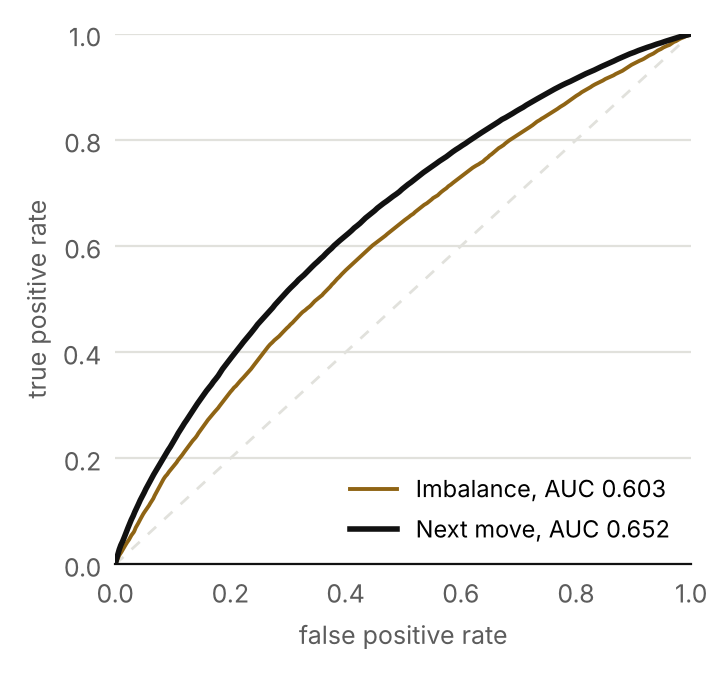
\includegraphics[width=0.42\linewidth]{roc.png}
\caption{ROC for the next mid move on the test afternoon. The model's curve lies above imbalance's everywhere. The most important features by permutation are 1-second trade imbalance, the size at the best ask, time since the last move, the size at the best bid, and 100-ms order-flow imbalance.}
\label{fig:roc}
\end{figure}

\section{Market making}\label{sec:mm}
\paragraph{Simulator.} The market maker quotes 100 shares at the best bid and ask from 9:35 to 15:55, skews one cent further back per 200 shares of inventory, and earns an assumed \dol0.0020 per share rebate for adding liquidity. Its quotes are shadow orders: they sit in a virtual queue among the real orders without changing them. Because ITCH names every order, the simulator knows exactly which real orders are ahead of a quote when it is placed. A quote fills when the orders ahead of it trade or cancel and a later execution reaches its price, when the market trades through it, or when a new order is priced through it. Placing and cancelling take effect after a configurable latency.

\paragraph{Filters.} A filter withdraws a quote (or moves it one cent back) when it expects that quote to be run over. \emph{Imbalance} pulls the ask when best-level imbalance is strongly positive, and the bid when strongly negative. \emph{Next move} does the same with the model's probability that the next move is up. \emph{Latency-trained} uses the model trained on the latency-aware label. \emph{Toxicity} predicts the one-second markout of a fill on each side, trained on the fills the unfiltered market maker received in the morning, and pulls a side when that markout is predicted to be poor.

\paragraph{Fair comparison.} Any filter that fires more often trades less, and since the unfiltered strategy loses money, trading less alone reduces the loss. Each filter's threshold is therefore set so that it fires a given share of the time on the tuning hour (10\% to 60\%), and filters are compared at the same activity. The activity rate itself is also chosen on the tuning hour.\footnote{An earlier version of the accompanying site reported a profit of \dol160 at zero latency. That rate had been chosen by looking at the test afternoon; chosen on the tuning hour, the result is the $-\dol470$ reported here.}

\begin{figure}[t]
\centering
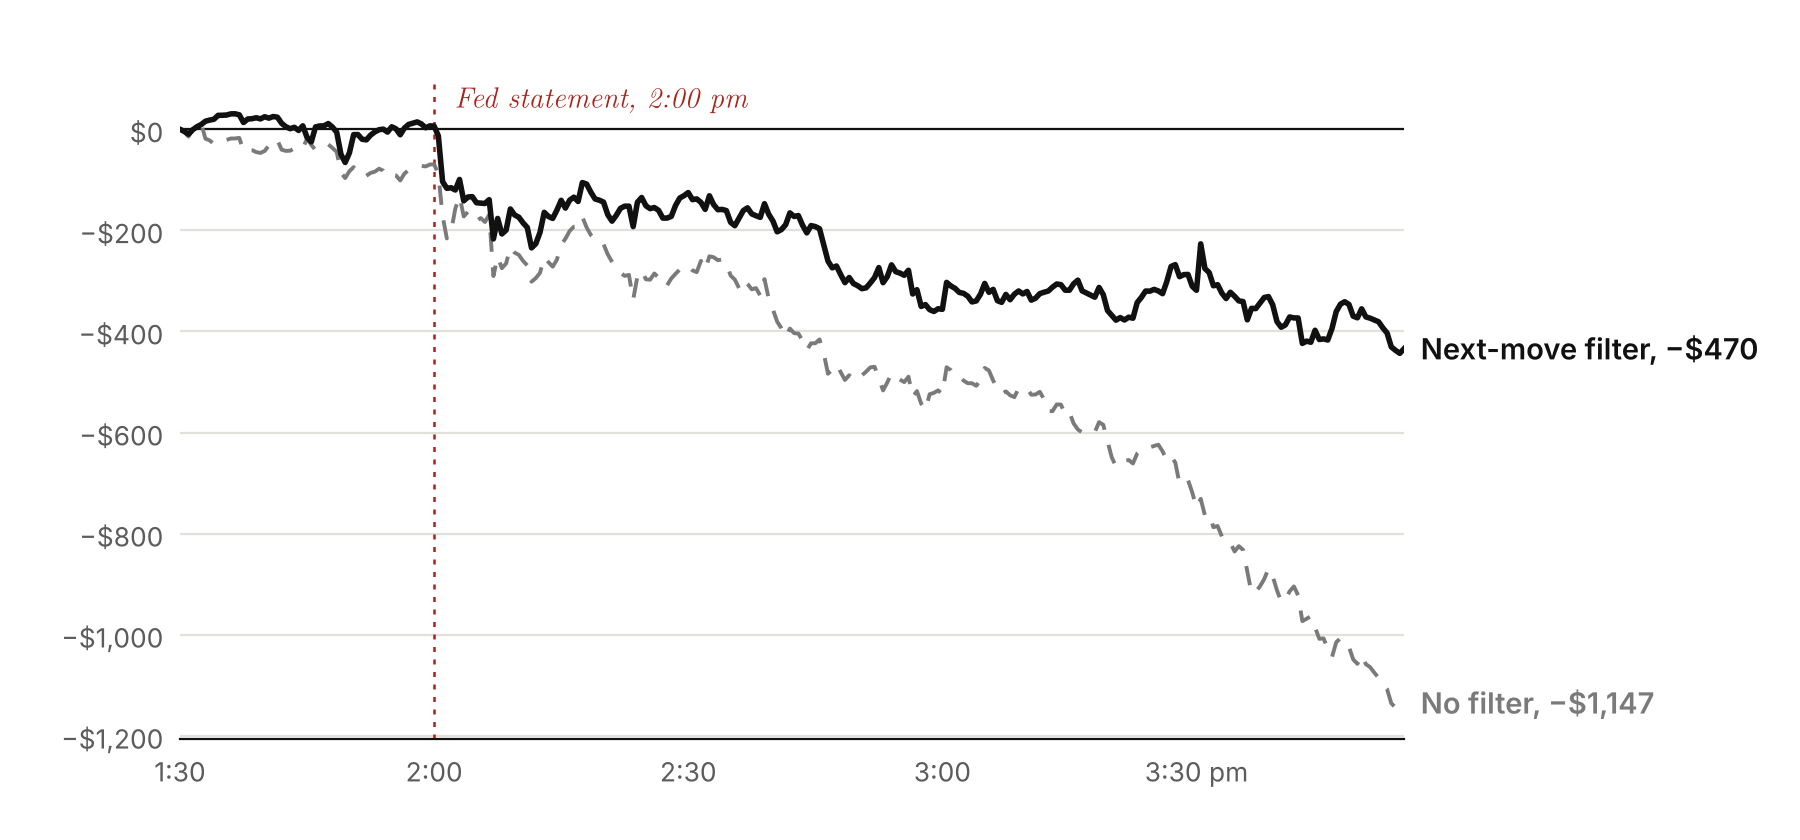
\includegraphics[width=0.92\linewidth]{headline.png}
\caption{Running PnL with rebate on the test afternoon, zero latency. Solid: the next-move filter, pulling quotes 20\% of the time, the rate chosen on the tuning hour. Dashed: no filter. The gap opens at the Federal Reserve statement at 2:00~pm, when the unfiltered quotes are run over repeatedly.}
\label{fig:pnl}
\end{figure}

\begin{table}[t]
\centering\small
\begin{tabular}{lrrrrr}
\toprule
Latency & No filter & Imbalance & Next move & Latency-trained & Toxicity \\
\midrule
0 & $-\dol1{,}147$ & $-\dol841$ & $-\dol470$ & -- & $\mathbf{-\dol440}$ \\
100 \textmu s & $-\dol2{,}086$ & $-\dol1{,}425$ & $-\dol1{,}370$ & $\mathbf{-\dol835}$ & $-\dol917$ \\
1 ms & $-\dol2{,}792$ & $-\dol2{,}161$ & $-\dol1{,}498$ & $-\dol1{,}491$ & $\mathbf{-\dol1{,}371}$ \\
10 ms & $-\dol3{,}325$ & $-\dol2{,}610$ & $-\dol2{,}270$ & $\mathbf{-\dol1{,}303}$ & $-\dol2{,}037$ \\
\bottomrule
\end{tabular}
\caption{PnL with rebate on the test afternoon, each filter pulling quotes at the activity rate chosen on the tuning hour. At zero latency the latency-trained model is the next-move model. The best ML filter loses 51--62\% less than quoting blindly at every latency; imbalance saves 22--32\%.}
\label{tab:mm}
\end{table}

\begin{figure}[t]
\centering
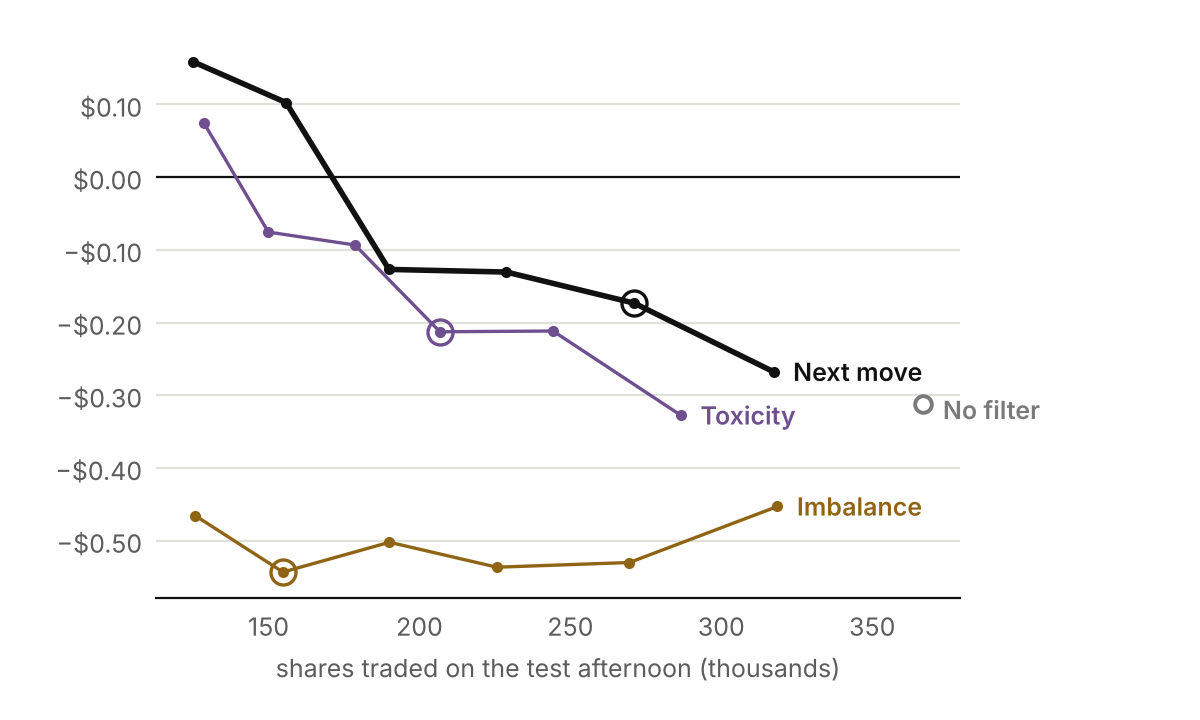
\includegraphics[width=0.66\linewidth]{frontier.png}
\caption{Edge, or just less trading? Loss per 100 shares against shares traded at zero latency, one line per filter as its activity rate runs from 10\% to 60\%; circled points are the tuning-hour choices. Imbalance trades less but loses \emph{more} per share than quoting blindly; the ML filters lose less per share at the same volume. Across all latencies, actions and placements, ML filters beat imbalance per share in 126 of 132 matched settings.}
\label{fig:frontier}
\end{figure}

Table~\ref{tab:mm} and Figure~\ref{fig:frontier} give the results. Two findings stand out. First, imbalance reduces the loss mainly by trading less: at zero and 100~\textmu s latency it loses more per share than quoting blindly, because the quotes it keeps are the ones the crowd is already leaning away from. Second, as latency grows the plain next-move model degrades and the models built for it take over: the latency-trained model at 100~\textmu s and 10~ms, the toxicity model at 1~ms.

\section{Away from the test afternoon}\label{sec:robust}
\paragraph{A second day.} On 30 December 2019 every model, threshold and activity rate is applied exactly as fixed on 30 January; nothing is refit. The next-move model's AUC is 0.648 against 0.605 for imbalance (interval $+0.039$ to $+0.046$), and the 100~\textmu s model holds similarly (0.625 against 0.593). The 1 and 10~ms models do not: their gains vanish (Table~\ref{tab:day2}). In the backtest the toxicity filter loses least at every latency, cutting the day's loss by 40--72\% against quoting blindly.

\begin{table}[h]
\centering\small
\begin{tabular}{lrrrrr}
\toprule
Latency & No filter & Imbalance & Next move & Latency-trained & Toxicity \\
\midrule
0 & $-\dol3{,}037$ & $-\dol2{,}170$ & $-\dol2{,}138$ & -- & $\mathbf{-\dol900}$ \\
100 \textmu s & $-\dol4{,}016$ & $-\dol3{,}091$ & $-\dol3{,}514$ & $-\dol2{,}484$ & $\mathbf{-\dol1{,}130}$ \\
1 ms & $-\dol8{,}378$ & $-\dol6{,}675$ & $-\dol6{,}270$ & $-\dol6{,}079$ & $\mathbf{-\dol4{,}983}$ \\
10 ms & $-\dol11{,}029$ & $-\dol8{,}882$ & $-\dol8{,}794$ & $-\dol6{,}793$ & $\mathbf{-\dol6{,}644}$ \\
\midrule
AUC, next move & & 0.605 & 0.648 & & \\
AUC, 1 ms label & & 0.572 & 0.574 & & \\
\bottomrule
\end{tabular}
\caption{30 December 2019, the whole day (9:35--15:55), with everything frozen from 30 January; each filter pulls quotes at its day-1 activity rate.}
\label{tab:day2}
\end{table}

\paragraph{Other stocks.} The same protocol on five other stocks on 30 January gives own-model AUCs of 0.734 (MSFT), 0.710 (INTC), 0.700 (SPY), 0.639 (NVDA) and 0.595 (AMZN), each above imbalance with intervals excluding zero. The AAPL model applied unchanged does not carry over to the one-tick stocks (INTC: 0.590 against 0.676 for imbalance), so the pattern is stock-specific even if the recipe is not.

\paragraph{SPY as a leading signal.} Adding SPY's order-flow features to Apple's model changes test AUC by $-0.001$ (interval $-0.004$ to $+0.002$): at these horizons Apple's own book already contains what SPY knows.

\section{Inference next to the engine}
The features and trees are reimplemented in C++ and run on the same rebuilt book. Over 1{,}441{,}976 decisions the C++ features and probabilities are bit-identical to Python's, which required computing logarithms through the same C math library on both sides. The full tuned model (300 trees of depth up to 25) costs 7.3~\textmu s per prediction; a 50-tree, depth-6 model keeps nearly all of the AUC (0.650 against 0.652) at 405~ns, and features cost 264~ns per decision.

\section{Limitations}
\begin{itemize}
\item Two days of one stock for the backtests. The second is a genuine out-of-sample test, but two days are not a track record.
\item Shadow orders have no market impact, so fill counts are optimistic; the rebate is assumed rather than taken from a fee schedule; auction and hidden-order fills are not modelled.
\item The tuning hour is short, so the activity rate it picks is noisy. That is the price of not choosing it on the test data.
\end{itemize}

\section{Conclusion}
A model of the next price move built from the public order book carries real information beyond book imbalance, and the information survives a held-out afternoon, a frozen second day and five other stocks. As a quote filter it roughly halves a passive market maker's loss at every latency tested, and does so by avoiding toxic fills rather than by trading less. It does not make passive market making on Apple profitable for a participant without queue priority or a better fee tier. Code, data pipeline and the interactive version of every result are at \href{https://github.com/adamdn-code/orderbook}{github.com/adamdn-code/orderbook}.

\end{document}
